\section{Build}\label{sec:build}
This section outlines the different build steps required to produce the final
system image containing the Muen separation kernel and all subjects as defined
by the system policy. Figure \ref{fig:build-process} illustrates the build
process.

\begin{figure}[h]
	\centering
	\begin{tikzpicture}[minimum height=0.6cm]
	\node (src) [apribox]               {Source Format};
	\node (mrg) [bluebox, right=of src] {Merger};
	\node (exp) [bluebox, right=of mrg] {Expander};
	\node (fma) [apribox, right=of exp] {Format A};
	\node (alo) [bluebox, right=of fma] {Allocator};
	\node (fmb) [apribox, below=of alo] {Format B};
	\node (val) [bluebox, left=of fmb]  {Validator};
	\node (sge) [bluebox, left=of val]  {Structure Generators};

	\node (spk) [graybox, below=of sge] {Source Specs};
	\node (iob) [graybox, right=of spk] {I/O Bitmaps};
	\node (msc) [graybox, right=of iob, minimum width=1.5cm] {...};
	\node (pta) [graybox, left=of spk] {Page Tables};
	\node (zpa) [graybox, left=of pta] {Zero Page};

	\node (bin) [apribox, below=of spk] {Binaries};

	\node (has) [bluebox, below=of bin] {Hasher};

	\node (sin) [bluebox, below=of has] {Sinfo};

	\node (pak) [bluebox, below=of sin] {Packer};

	\node (img) [apribox, below=of pak] {System Image};

	\draw[arrow] (src) -- (mrg);
	\draw[arrow] (mrg) -- (exp);
	\draw[arrow] (exp) -- (fma);
	\draw[arrow] (fma) -- (alo);
	\draw[arrow] (alo) -- (fmb);
	\draw[arrow] (fmb) -- (val);
	\draw[arrow] (val) -- (sge);

	\draw[arrow] (sge) -- (spk);
	\draw[arrow] (sge) -- (iob);
	\draw[arrow] (sge) -- (msc);
	\draw[arrow] (sge) -- (pta);
	\draw[arrow] (sge) -- (zpa);

	\draw[arrow] (spk) -- (bin);

	\draw[arrow] (bin) -- (has);
	\draw[arrow] (has) -- (sin);
	\draw[arrow] (sin) -- (pak);

	\draw[arrow] (msc) -- (pak);
	\draw[arrow] (iob) -- (pak);
	\draw[arrow] (iob) -- (pak);
	\draw[arrow] (pta) -- (pak);
	\draw[arrow] (zpa) -- (pak);

	\draw[arrow] (pak) -- (img);
\end{tikzpicture}

	\caption{Build process}
	\label{fig:build-process}
\end{figure}

The first step is to build the tools. The \texttt{skconfig} helper tool
outlined in section \ref{subsec:subject-binary-analysis} can be used to create
subject initial state and memory layout specifications in XML format based on
the subject binary. The generated XML files are included in the system policy
prior to the policy compilation step.

To compile the system policy, the \texttt{skpolicy} tool is required. The
details about the policy compilation process is described in section
\ref{subsec:policy-compilation}. The Muen kernel and all subjects depend on the
Ada ZFS runtime. Once the policy has been generated and the ZFS runtime has
been compiled, the kernel and all subjects are built.

The final step is to package all object binaries (i.e. the kernel and all
subjects) including all related files into a bootable OS image. This task is
handled by the \texttt{skpacker} tool described in section
\ref{subsec:image-packaging}.

To allow fast round-trips during kernel development, the Muen project uses
an emulator to directly boot the generated OS image after the build process is
complete. Section \ref{subsec:emulation} outlines the details about the
emulation facility.

The complete system build, deployment and emulation process is automated using
GNU Make \cite{make}. The top-level project Makefile provides targets to
perform the following tasks:

\begin{itemize}
	\item Compile all tools
	\begin{itemize}
		\item \texttt{make skconfig}
		\item \texttt{make skpolicy}
		\item \texttt{make skpacker}
	\end{itemize}
	\item Compile the Ada ZFP RTS
	\begin{itemize}
		\item \texttt{make rts}
	\end{itemize}
	\item Compile the policy
	\begin{itemize}
		\item \texttt{make policy}
	\end{itemize}
	\item Compile example system subjects
	\begin{itemize}
		\item \texttt{make subjects}
	\end{itemize}
	\item Compile Muen kernel
	\begin{itemize}
		\item \texttt{make kernel}
	\end{itemize}
	\item Package OS image
	\begin{itemize}
		\item \texttt{make pack}
	\end{itemize}
	\item Deploy OS image to actual hardware
	\begin{itemize}
		\item \texttt{make deploy}
	\end{itemize}
	\item Start emulation
	\begin{itemize}
		\item \texttt{make emulate}
	\end{itemize}
\end{itemize}

\subsection{Subject Binary Analysis}\label{subsec:subject-binary-analysis}
The \texttt{skconfig} tool uses the Binary File Descriptor (BFD\index{BFG})
library to analyze subject binaries and creates appropriate XML\index{XML}
policy specifications from it, see figure \ref{fig:object-analysis}. This is
useful to generate the initial state and the memory layout directly from a
native subject binary instead of writing it by hand. The tool extracts stack
address, entry point and memory layout from a subject binary.

\begin{figure}[h]
	\centering
	\begin{tikzpicture}
	\node (obj) [bluebox]                {Binary object};
	\node (skc) [apribox,  below=of obj] {skconfig};
	\node (xml) [greenbox, below=of skc] {XML specification};

	\draw[arrow] (obj) to (skc);
	\draw[arrow] (skc) to (xml);
\end{tikzpicture}

	\caption{From binary object to XML specification}
	\label{fig:object-analysis}
\end{figure}

The extracted subject initial state and memory layout XML specifications can be
included in the system policy before compilation by the \texttt{skpolicy} tool.
The generated memory layout is only as permissive as required by the original
subject binary. For example, the memory region mapped for executable code
(the \texttt{.text} section) will be executable but non-writable. This is in
contrast to just providing a big enough memory region granting all permissions
to the subject with no exact mapping of binary sections to memory access
permissions (i.e. read, write, execute).

\subsection{Policy Compilation}\label{subsec:policy-compilation}
The \texttt{skpolicy} tool compiles the XML system policy to different output
formats as shown in figure \ref{fig:policy-compilation}.

\begin{figure}[h]
	\centering
	\begin{tikzpicture}
	\node (pol) [greenbox]                            {Policy};
	\node (skp) [apribox, below=of pol]               {skpolicy};
	\node (sou) [bluebox, below=of skp, xshift=1.5cm] {Source specs};
	\node (pag) [bluebox, left=of sou]                {Page tables};
	\node (iob) [bluebox, left=of pag]                {I/O bitmaps};
	\node (msr) [bluebox, right=of sou]               {MSR bitmaps};

	\draw[arrow] (pol) to (skp);
	\draw[arrow] (skp) to (sou);
	\draw[arrow] (skp) to (msr);
	\draw[arrow] (skp) to (pag);
	\draw[arrow] (skp) to (iob);
\end{tikzpicture}

	\caption{Policy compilation}
	\label{fig:policy-compilation}
\end{figure}

The generated page tables, I/O and MSR bitmaps are included in the final system
image by the \texttt{skpacker} utility. These files are all in binary form and
correspond to the format mandated by the respective Intel SDM chapters
\cite{IntelSDM}. Page tables are generated for subjects as well as for the
kernel itself.

The generated SPARK and Assembly source specifications are included in the
kernel directly. These specifications provide the kernel with the following
information:

\begin{itemize}
	\item \emph{IRQ routing specification}\\
		Used by the kernel to program the system's I/O APIC for interrupt
		routing.
	\item \emph{Vector routing specification}\\
		Used by the kernel to determine the destination subject of interrupt
		vectors.
	\item \emph{Kernel address constants}\\
		Define kernel stack, page table and per-CPU storage memory addresses.
	\item \emph{Scheduling plans for all CPU cores}\\
		The scheduling plans are indexed by the logical processor's APIC ID.
		Each kernel copies its associated scheduling plan to the per-CPU storage
		area on initialization.
	\item \emph{Subject specifications}\\
		Defines all subjects and their parameters, see policy section
		\ref{subsec:subjects}.
	\item \emph{Packer specification}\\
		Defines the configuration used for the \texttt{skpacker} tool.
\end{itemize}

\subsubsection{Validity Checks}
Before generating the source specifications, page tables and bitmaps, the policy
compiler performs various sanity checks to assert the validity of the system
policy. This is done in two steps. First, the policy is validated against the
Muen system schema. If this step fails, no further processing is performed and
the user is informed about the error. If the policy validates, the policy
compiler performs additional validity checks in a second step:

\begin{itemize}
	\item Assert that all hardware device references are valid.
	\item Assert that event table entries have an unique event number.
	\item Assert that trap table entries have an unique exit reason.
	\item Assert that hardware device IRQs are unique.
	\item Assert that memory addresses used by the kernel are page aligned.
	\item Assert alignment of all memory regions in the policy.
	\item Assert that MSR address ranges are valid.
	\item Assert that every subject referenced in the scheduling plan exists.
	\item Assert that subjects are scheduled on the correct logical CPU.
	\item Assert that the scheduling plan contains a major frame for each CPU.
	\item Assert that a specific major frame has equal tick count on all logical
		CPUs.
	\item Disallow subject self-references in the event table.
	\item Assert that every subject referenced in a subject's event table exists.
	\item Assert that handover event destination subjects run on the same CPU.
	\item Disallow IPI for interrupt events on the same CPU.
	\item Disallow subject self-references in the trap table.
	\item Assert that every subject referenced in a subject's trap table does
		exist.
	\item Assert that trap destination subjects run on the same CPU.
	\item Assert that all memory addresses used to setup a subject are page
		aligned.
	\item Assert that subject binary references are valid.
\end{itemize}

\subsection{Image Packaging}\label{subsec:image-packaging}
The \texttt{skpacker} tool is responsible to assemble the final bootable system
image from the parts produced in the preceding build steps. Figure
\ref{fig:image-packaging} illustrates the process. The tool includes the packer
relevant source specification created from the system policy. This specification
provides information about subject binaries and their physical address in the
final image.

\begin{figure}[h]
	\centering
	\begin{tikzpicture}
	\node (knl) [bluebox]                              {Kernel binary};
	\node (sub) [bluebox, left=of knl]                 {Subject binaries};
	\node (pag) [bluebox, left=of sub]                 {Page tables};
	\node (bit) [bluebox, right=of knl]                {Bitmaps};
	\node (skp) [apribox, below=of knl, xshift=-1.5cm] {skpacker};
	\node (spe) [bluebox, left=of skp]                 {Packer spec};
	\node (sys) [greenbox, below=of skp]               {System image};

	\draw[arrow] (pag) to (skp);
	\draw[arrow] (sub) to (skp);
	\draw[arrow] (knl) to (skp);
	\draw[arrow] (bit) to (skp);
	\draw[arrow] (skp) to (sys);
	\draw[arrow] (spe) to (skp);
\end{tikzpicture}

	\caption{System image packaging}
	\label{fig:image-packaging}
\end{figure}

The remaining configuration information is extracted from the source
specification provided to the kernel. Listing \ref{lst:skpacker} shows the
output of a \texttt{skpacker} run with the example system described in section
\ref{sec:example-system}. The first column in the output designates physical
memory addresses in hexadecimal form. The second column specifies the type of
the packaged file at this specific memory location. The abbreviations have the
following meaning:

\begin{description}
	\item[PML4] The file at this address designates a page table structure. It
		is either a page table for a kernel or for a subject. The kernels
		running on the different logical processors have different page tables
		to allow distinct stack and per-CPU storage pages transparently.
	\item[IOBM] The file is a subject I/O bitmap. It specifies which I/O ports a
		subject is allowed to access.
	\item[MSBM] The file is a subject MSR bitmap. It specifies which MSRs a
		subject is allowed to access.
	\item[BIN] The file is a subject binary.
\end{description}

\begin{lstlisting}[
	caption=Example output of skpacker tool,
	label=lst:skpacker,
	frame=none,
	numbers=none]
         Packaging kernel image 'obj/kernel'
         0000000000200000 [PML4] kernel (0)
         0000000000204000 [PML4] kernel (1)
         0000000000208000 [PML4] kernel (2)
         000000000020c000 [PML4] kernel (3)
         0000000000210000 [PML4] tau0
         0000000000214000 [IOBM] tau0
         0000000000216000 [MSBM] tau0
         0000000000217000 [BIN ] tau0
         0000000000240000 [PML4] vt
         0000000000244000 [IOBM] vt
         0000000000246000 [MSBM] vt
         0000000000247000 [BIN ] vt
         0000000000270000 [PML4] crypter
         0000000000274000 [IOBM] crypter
         0000000000276000 [MSBM] crypter
         0000000000277000 [BIN ] crypter
         00000000002a0000 [PML4] sm
         00000000002a4000 [IOBM] sm
         00000000002a6000 [MSBM] sm
         00000000002a7000 [BIN ] sm
         00000000002d0000 [PML4] xv6 (EPT)
         00000000002d4000 [IOBM] xv6
         00000000002d6000 [MSBM] xv6
         00000000002d7000 [BIN ] xv6
\end{lstlisting}

Once the packaging step is complete, the resulting OS image can be booted by any
Multiboot \cite{multiboot} compliant bootloader.

\subsection{Emulation}\label{subsec:emulation}
To ease kernel development, the Muen project makes use of emulation by employing
the Bochs IA-32 emulator. Among many other features, Bochs has support for
multiple processors, APIC emulation and VMX extensions. Figure \ref{fig:bochs}
shows the Bochs emulator running the Muen example system described in section
\ref{sec:example-system}.

\begin{figure}[h]
	\centering
	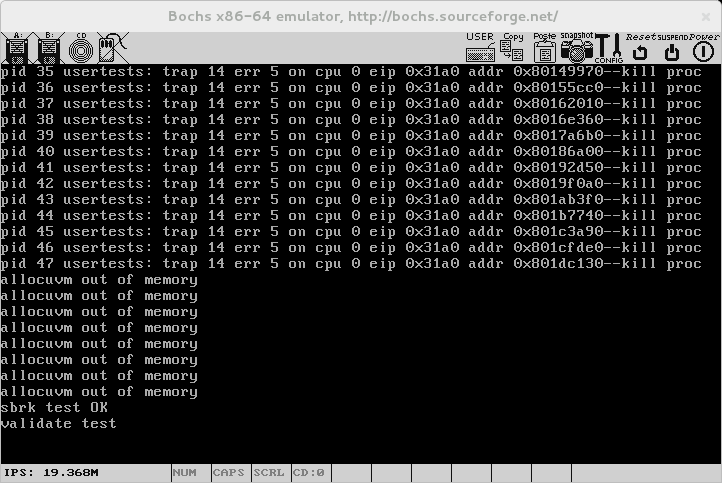
\includegraphics[width=\textwidth]{images/bochs}
	\caption{Bochs running the Muen example system}
	\label{fig:bochs}
\end{figure}

Bochs writes detailed logs during emulation and provides a debugger which allows
to inspect the complete system state at any time. It has proven very helpful
and was invaluable when implementing new low-level processor features.
